\subsection{Convolutional Layer}

The convolutional layer - referred to as conv2d - receives an input data tensor $X_{ci} $ of size $[H, W, C_{in}]$ and outputs a data tensor of size $[H,W,C_{out}]$. Here $H$ and $W$ is the height and width of the convolutional kernel. So every input tensor is transferred to each single convolutional computation channel, which is responsible for computing a \emph{single} output channel. Each convolutional channel is parameterized with its own set of values. Those values are implemented as constants in VHDL, which has the advantages of greater optimization options by the compiler as well as reduced data movement. Therefore template entities are created for the convolution channel- and layer entities where the weights are then populated via a Python script.

\begin{figure}[hb]
	\centering
	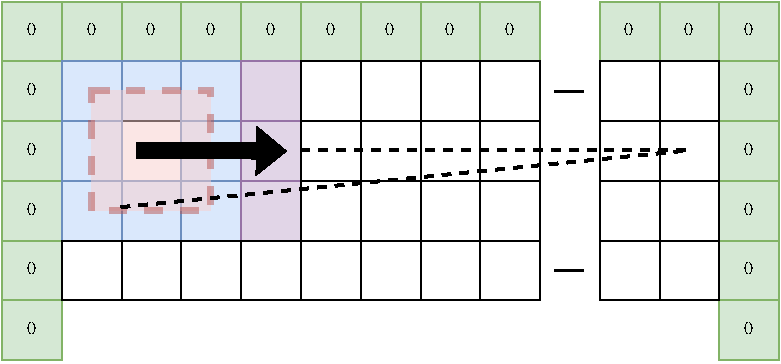
\includegraphics[width=0.6\textwidth]{img/convolution.pdf}
	\caption[Convolution Operation]{Convolution Operation. The convolutional kernel (red-dashed-square) is shifted over the input data. The currently processed data is shown in blue and the only three pixels (violett) need to be loaded for the next convolution because of data reuse. Note that for the convolution operation the image must be padded (in our case by zeros) to sustain image dimensions. Depth channels omitted for illustration purposes.}
	\label{fig:hw-conv-operation}
\end{figure}

The principal operation can be shown in Figure~\ref{fig:hw-conv-operation}. Here the convolutional kernel slides over the input data from left to right, top to bottom. It can be seen that most of the $6$ of $9$ input pixels (of each input channel) can be reused. This is done via shift registers and because all weights of the kernel remain unchanged for the operation this results in minimum data movement. Note that for the convolutional operations the input data must be padded in order to sustain the image dimensions.


\begin{figure}[h]
	\centering
	\begin{subfigure}[t]{0.5\textwidth}
		\centering
		% Constrain the height instead of the widht so the images are equally aligned at the top
		\includesvg[height=2.5in]{img/inkscape/conv2d.svg}
		\caption[Conv2d block diagram.]{Conv2d block diagram. For each output channel a conv\_channel module is used. $k$ indicates the number of output channels.}
		\label{fig:conv2d}
	\end{subfigure}%
	~
	\begin{subfigure}[t]{0.5\textwidth}
		\centering
		\includesvg[height=2.5in]{img/inkscape/conv-channel.svg}
		\caption[conv\_channel block diagram.]{conv\_channel block diagram. For each input channel a kernel\_3x3 module is used. $n$ indicates the number of input channels.}
		\label{fig:conv-channel}		
	\end{subfigure}
	\caption{Block diagram of the Convolutional Layer}
	\label{fig:hw-layer-conv}
\end{figure}


In Figure~\ref{fig:conv2d} the block diagram of the top-level conv2d module is shown. It consists of $k$ conv\_channel modules to realise $k$ output channels. All conv\_channel modules recieve the same input vector $X_{c_i}$. 
The internal structure of a conv\_channel module is shown in Figure \ref{fig:conv-channel}. It uses $n$ kernel\_3x3 modules to realise $n$ input channels. All kernel\_3x3 modules get a different input vector $X_{c_{i1}}$ to $X_{c_{in}}$ which are $3 \times 3$ input matrices. All kernel outputs are summed up to one final value of length BIT\_WIDTH\_OUT.

\subsubsection{Interface}

\begin{itemize}
	\item Input interface connected to shift register, which consists of a $n \cdot 3 \times 3$ vector of values of length BIT\_WIDTH\_IN, in which $n$ is the number of input channels.
	\item Output interface connected to the pooling layer, which is a vector of $m$ values of length BIT\_WIDTH\_OUT, in which $m$ is the number of output channels.
\end{itemize}
Both input and output interfaces have ready, last and valid signals to control the flow of data.

\subsubsection{Parameter}

\begin{table}[hb]
	\centering
	\begin{tabular}{lcc}
		\toprule
		Parameter & VHDL Datatype & Type \\
		\midrule
		 BIT\_WIDTH\_IN & integer & Generic\\
		 BIT\_WIDTH\_OUT & integer & Generic \\
		 INPUT\_CHANNELS & integer & Generic\\
 	 	 OUTPUT\_CHANNELS & integer & Generic \\
		\bottomrule
	\end{tabular}
\end{table}




\subsubsection*{conv\_channel}


\textbf{Interface}
\begin{itemize}
	\item Input interface, same as conv2d.
	\item Output interface connected to the pooling layer, which is a value of length BIT\_WIDTH\_OUT.
\end{itemize}

\textbf{Parameter}
\begin{itemize}
 	\item BIT\_WIDTH\_IN : integer
 	\item KERNEL\_WIDTH\_OUT : integer, output bit width of the kernel\_3x3 module
 	\item BIT\_WIDTH\_OUT: integer
 	\item N: integer, number of kernels
 	\item OUTPUT\_MSB: integer, defines which of the $n$=BIT\_WIDTH\_OUT bits is the most significant bit
 	\item BIAS: integer, currently unused as bias seems to not be very important in the convolutional layers
\end{itemize}
